% cap4.tex

\chapter{Análisis de Resultados}
\label{c4} % la etiqueta para referencias

\section{Resultados Replicación modelo original en Julia}

SE ME OCURRE PONER ACA LOS RESULTADOS DE REPLICAR EL MODELO EN JULIA Y COMPARAR CON GAMS, RENDIMIENTO, RESULTADOS.

\section{Aplicación de atención racional en el subastador}

En el capítulo anterior se aplica el concepto de atención racional en el modelo del subastador. Esta implementación es primero realizada en \ref{modelo:conrendimiento}, basada en \cite{dewan_estimating_2020}, al agregar un rendimiento de obtención de ingreso (en este caso el ingreso del subastador es la venta de permisos en la primera etapa), dependiente de cuanto dinero gasta en información adicional.
\vspace{2.5mm}

Para completar el modelo, se deben agregar los parámetros definidos en \ref{fig:nomenclatura1} sobre costos, capacidades instaladas, demandas en los periodos, factores de contaminación por tecnología, entre otros. Se utilizaron los aplicados en el modelo original de \cite{amigo_two_2021}. Sus valores específicos se encuentran en el Anexo \ref{anexo:parametros}.
\vspace{2.5mm}

En adición a esto, se deben definir los siguientes valores asociados al modelo del subastador con atención racional :

\begin{enumerate}
    \item Al igual que en la programación del modelo original, se considera el costo social independiente de los permisos  $\frac{\partial\mathcal{F}(\theta)}{\partial(\theta)}=0$
    \item $CAP\sim \mathcal{N}(100MtCO_{2}e,0)$
    \item Se definen las contantes del costo de rendimiento $c$ y $d$ explicadas en \ref{marco:costos}. Con esto, se decide utilizar los mismos valores que utilizaron los autores \citeB{dewan_estimating_2020}:
    \begin{enumerate}
        \item $d = 0.2$
        \item $c = 40$
    \end{enumerate}
\end{enumerate}

Con esto, al correr el modelo en el \textit{solver}, cambiando únicamente el valor del rendimiento ($P$), se encontraron los siguientes resultados:

\begin{table}[H]
\centering
\begin{tabular}{|l|l|l|}
\hline
\textbf{P($\%$)} & \textbf{$\theta$ (millones)} & \textbf{$\pi^a$($\frac{\$}{\theta}$)} \\ \hline
20 & 3203 & 0 \\ \hline
25 & 190 & 103.196 \\ \hline
30 & 204.63 & 73.335 \\ \hline
35 & 219.81 & 77.973 \\ \hline
40 & 219.79 & 60.880 \\ \hline
45 & 235.31 & 60.448 \\ \hline
50 & 379.72 & 77.507 \\ \hline
55 & 221.79 & 52.927 \\ \hline
60 & 230.75 & 48.799 \\ \hline
65 & 239.28 & 46.123 \\ \hline
70 & 248.33 & 49.598 \\ \hline
75 & 225.99 & 47.855 \\ \hline
80 & 235.93 & 62.802 \\ \hline
85 & 263.95 & 42.426 \\ \hline
90 & 272.16 & 41.955 \\ \hline
95 & 275.08 & 39.492 \\ \hline
100 & 328.44 & 38.110 \\ \hline
\end{tabular}
\caption{Resultados modelo con restricción de rendimiento}
\label{tabla:conrestrrend}
\end{table}

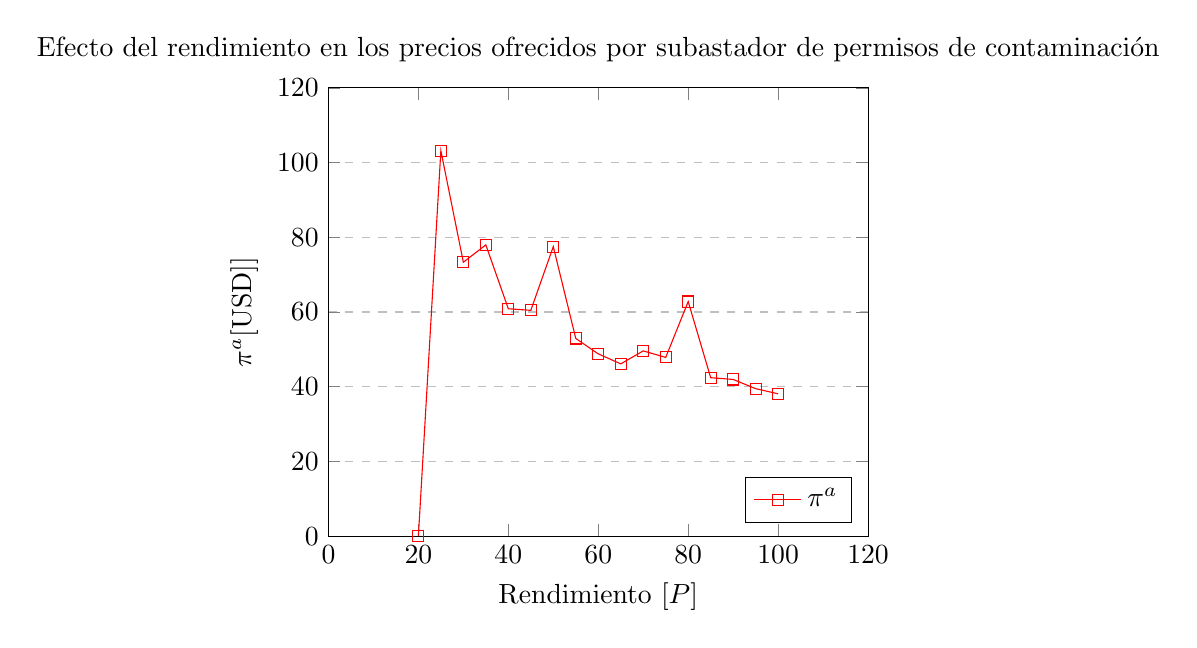
\begin{tikzpicture}
\begin{axis}[
    title={Efecto del rendimiento en los precios ofrecidos por subastador de permisos de contaminación},
    xlabel={Rendimiento [$P$]},
    ylabel={$\pi^a$[USD]]},
    xmin=0, xmax=120,
    ymin=0, ymax=120,
    xtick={0,20,40,60,80,100,120},
    ytick={0,20,40,60,80,100,120},
    legend pos=south east,
    ymajorgrids=true,
    grid style=dashed,
]

\addplot[
    color=red,
    mark=square,
    ]
    coordinates {
    (20,0)(25,103.196)(30,73.335)(35,77.973)(40,60.880)(45,60.448)(50,77.507)(55,52.927)(60,48.799)(65,46.123)(70,49.598)(75,47.855)(80,62.802)(85,42.426)(90,41.955)(95,39.492)(100,38.110)
    };
    \legend{$\pi^a$}
    
\end{axis}
\end{tikzpicture}

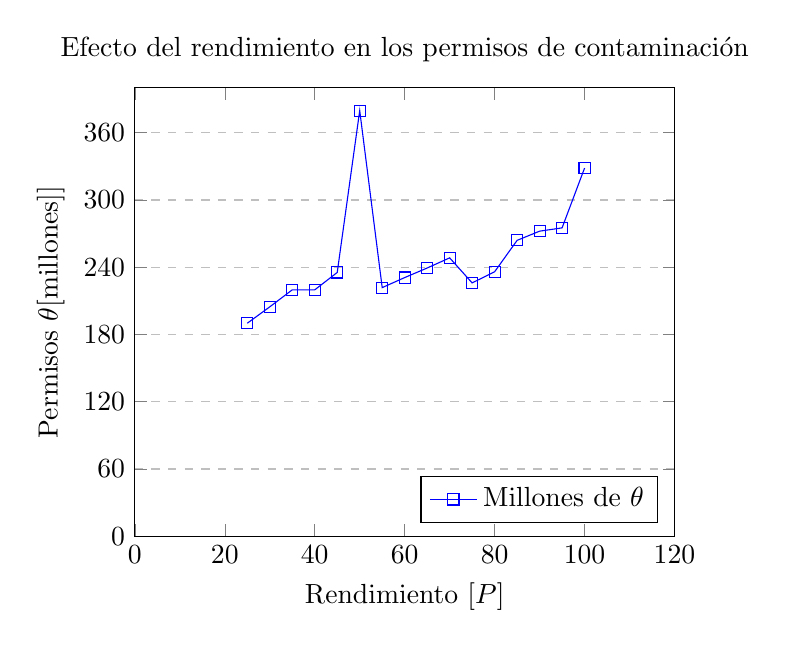
\begin{tikzpicture}
\begin{axis}[
    title={Efecto del rendimiento en los permisos de contaminación},
    xlabel={Rendimiento [$P$]},
    ylabel={Permisos $\theta$[millones]]},
    xmin=0, xmax=120,
    ymin=0, ymax=400,
    xtick={0,20,40,60,80,100,120},
    ytick={0,60,120,180,240,300,360},
    legend pos=south east,
    ymajorgrids=true,
    grid style=dashed,
]

\addplot[
    color=blue,
    mark=square,
    ]
    coordinates {
    (25,190)(30,204.63)(35,219.81)(40, 219.79)(45, 235.31)(50,379.72)(55,221.79)(60, 230.75)(65,239.28)(70,248.33)(75,225.99)(80,235.93 )(85,263.95)(90,272.16)(95,275.08)(100,328.44)
    };
    \legend{Millones de $\theta$}
    
\end{axis}
\end{tikzpicture}



